\documentclass[12pt]{amsart}
\usepackage{amsmath}
\usepackage{tikz,float,caption}
\usetikzlibrary{arrows.meta,calc,decorations.markings,patterns,cd,patterns.meta}

\begin{document}

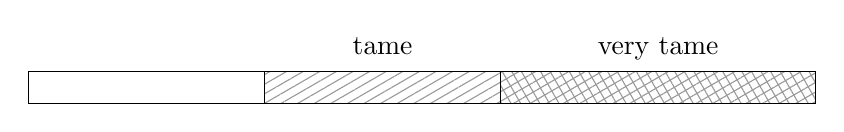
\begin{tikzpicture}[yscale=.4]
    \fill[pattern={Lines[angle=30]},pattern color=black!40!white] (3,0) rectangle (10,1);
    \fill[pattern={Lines[angle=-60]},pattern color=black!40!white] (6,0) rectangle (10,1);
    \path (3,2.4)--node[below]{tame}+(3,0);
    \path (6,2.4)--node[below]{very tame}+(4,0);
    \draw (0,0) rectangle (10,1) (3,0)--+(0,1) (6,0)--+(0,1);
  \end{tikzpicture}

\end{document}